\begin{frame}
  \frametitle{Multiphysics simulation results (2D)}
  \begin{figure}
   \vspace{-0.1in}
   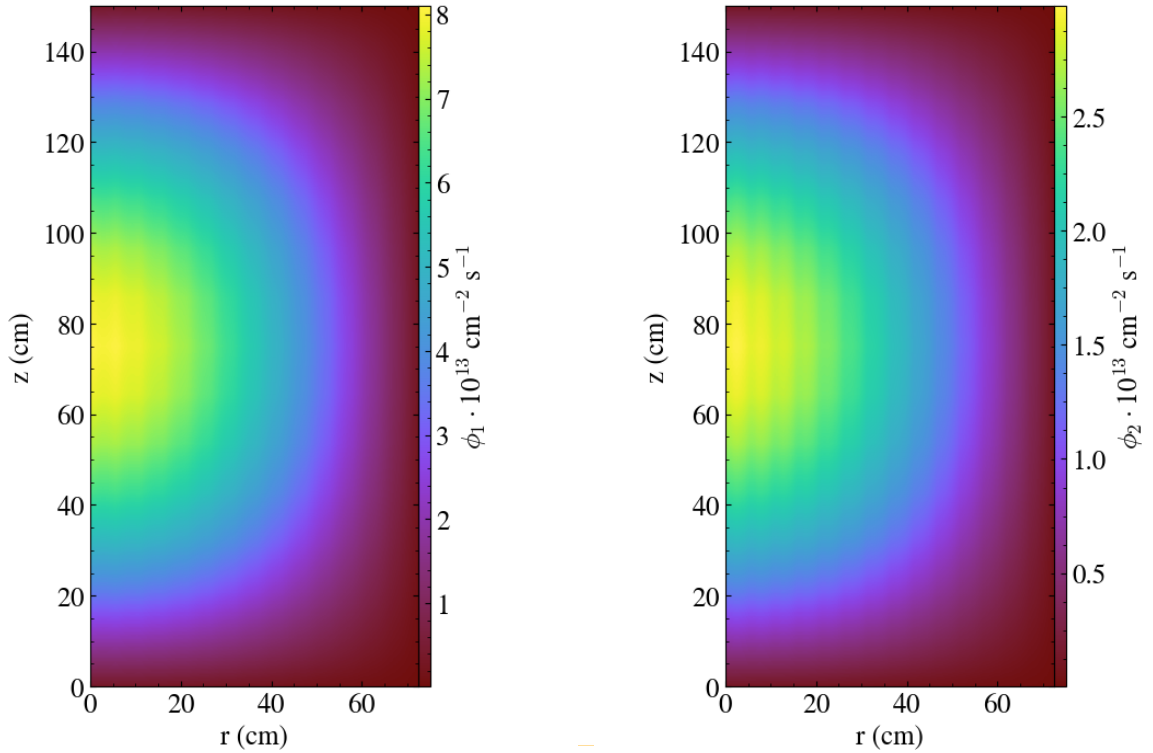
\includegraphics[height=0.85\textheight]{./images/moltres_flux.png}
   \vspace{-0.1in}
   \caption{Fast ($\phi_1$) and thermal ($\phi_2$) neutron flux obtained using Moltres 			\cite{lindsay_introduction_2018}.}
    \end{figure}
\end{frame}

\begin{frame}
  \frametitle{Multiphysics simulation results (2D) (2)}
  \begin{figure}[t]
   \vspace{-0.05in}
   \hspace*{-0.15in}
   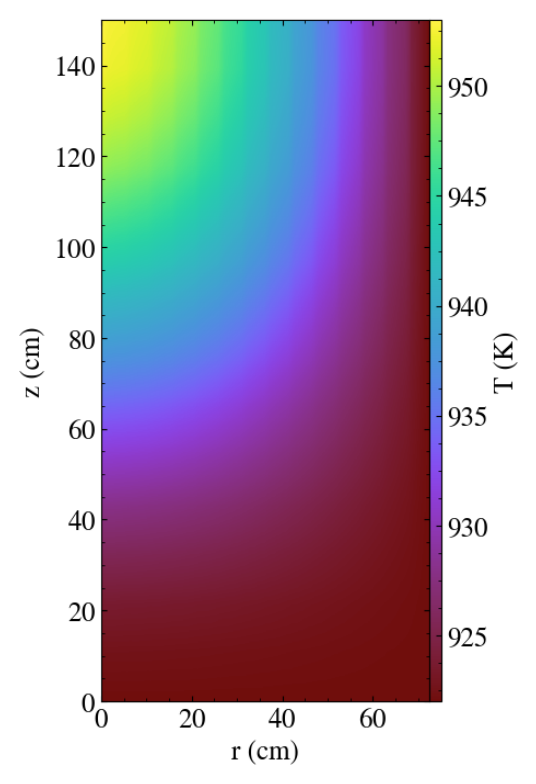
\includegraphics[height=0.85\textheight]{./images/moltres_temp.png}
   \vspace{-0.1in}
   \caption{Temperature in channel obtained using Moltres \cite{lindsay_introduction_2018}.}
    \end{figure}

\end{frame}

\begin{frame}
  \frametitle{Moltres vs MSRE Comparison}
  \begin{figure}[t]
   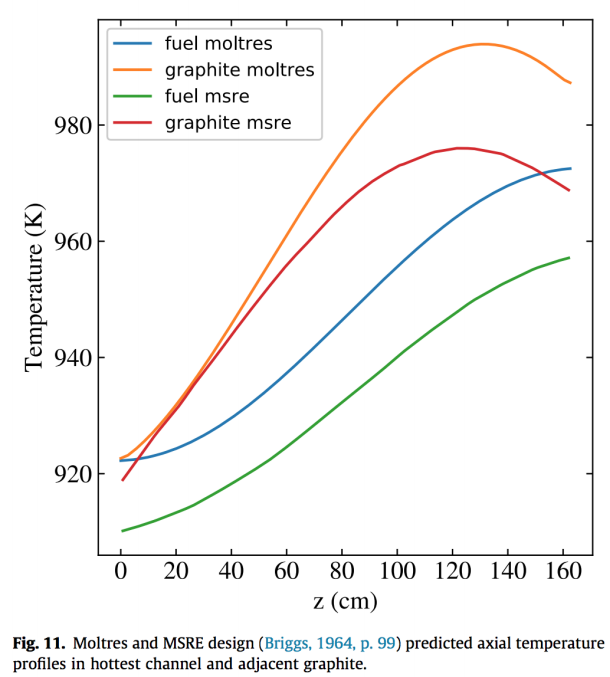
\includegraphics[height=0.85\textheight]{./images/msre_temp.png}
    \end{figure}

\end{frame}

\begin{frame}
  \frametitle{Moltres vs MSRE Comparison (2)}
  \begin{figure}[t]
   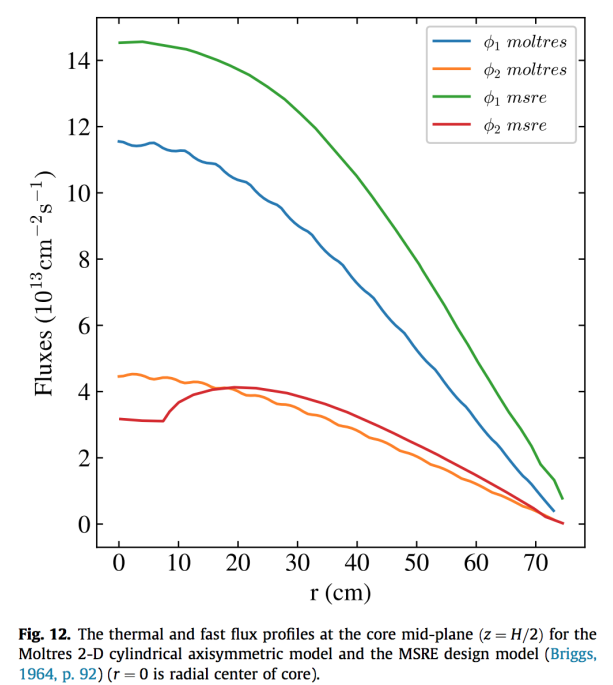
\includegraphics[height=0.85\textheight]{./images/msre_radial_flux.png}
    \end{figure}

\end{frame}

\begin{frame}
  \frametitle{Moltres vs MSRE Comparison (3)}
  \begin{figure}[t]
   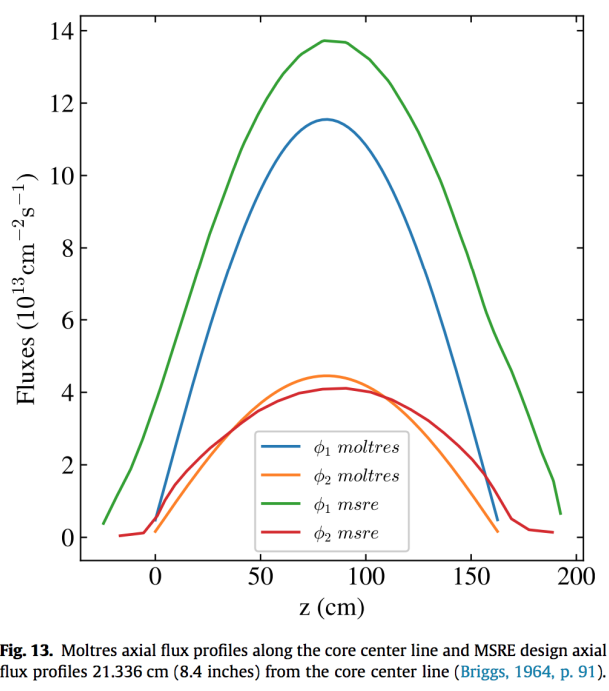
\includegraphics[height=0.85\textheight]{./images/msre_axial_flux.png}
    \end{figure}

\end{frame}

\begin{frame}
  \frametitle{Multiphysics simulation results (3D)}
  \begin{figure}[t]
   \vspace{-0.15in}
   \hspace*{-0.8in}
   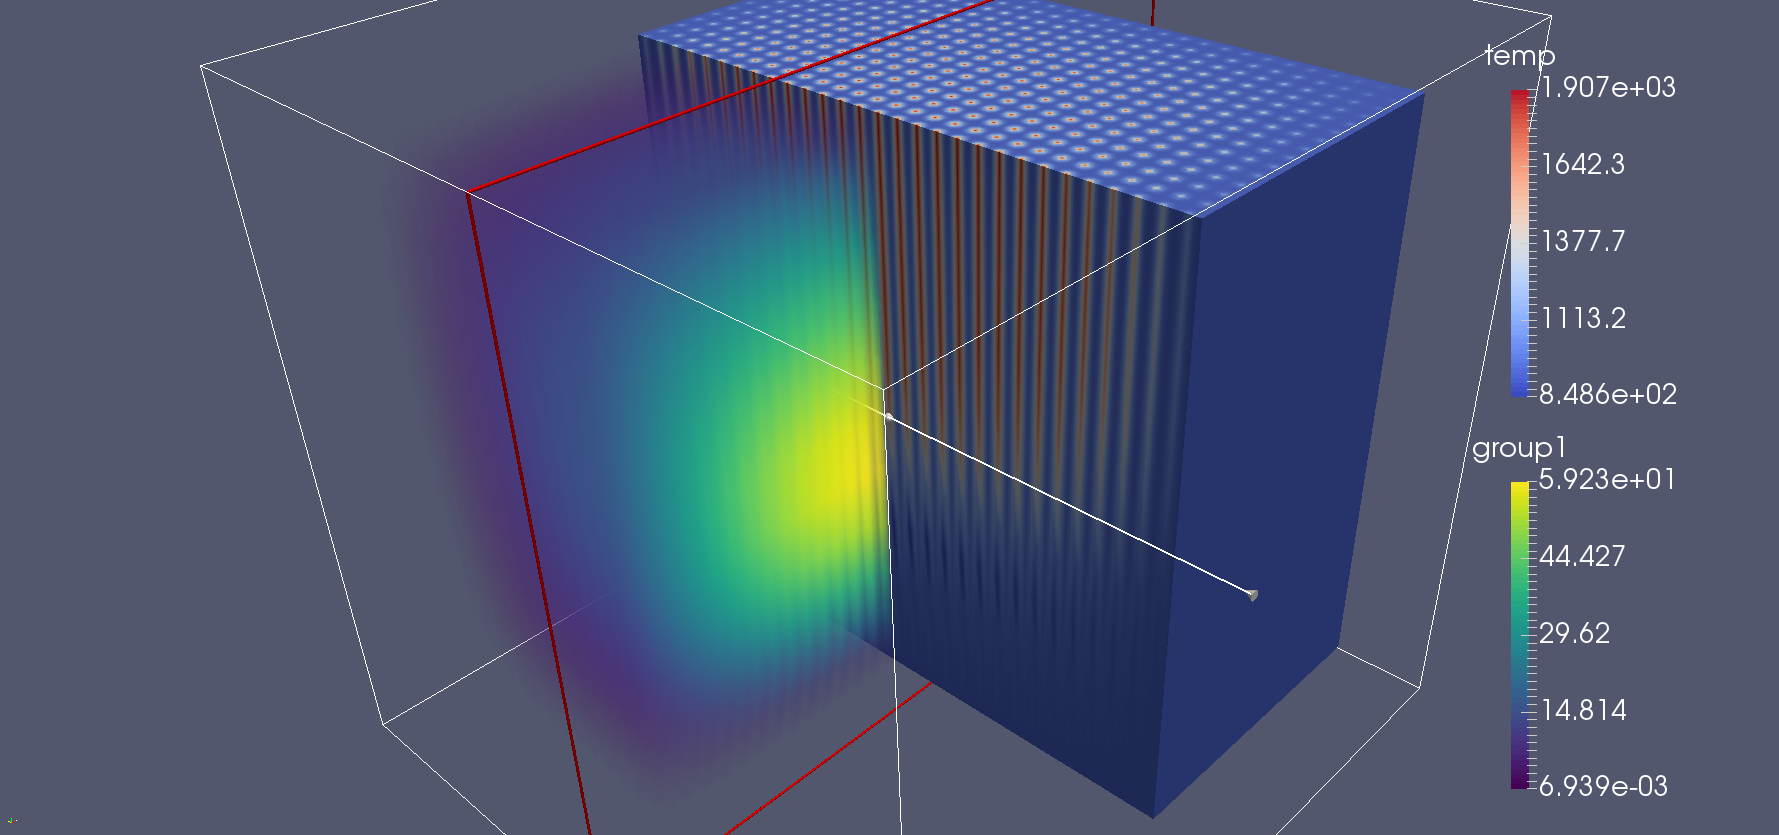
\includegraphics[height=0.8\textheight]{./images/moltres_3D.png}
   \caption{\gls{MSRE} steady-state temperature and fast neutron flux \cite{ridley_introduction_2017}.}
    \end{figure}
\end{frame}

%\begin{frame}
%\includemedia[
%  activate=pageopen,
%  width=540pt,height=400pt,
%  addresource=./videos/test.mp4,
%  flashvars={%
%     source=./videos/test.mp4% same path as in addresource!
%   &autoPlay=true%    % optional configuration
%   &loop=true%        % variables
%  }  
%]{}{APlayer.swf}
%\end{frame}